\chapter{ارزیابی و نتایج یادگیری}

در این فصل، نتایج حاصل از فرآیند یادگیری تقویتی در محیط سه‌جسمی ارائه و تحلیل شده است. هدف، بررسی عملکرد الگوریتم‌های استفاده‌شده و ارزیابی توانایی آن‌ها در دستیابی به اهداف تعیین‌شده می‌باشد.

\section{تنظیمات آزمایشی}

تنظیمات شبیه‌سازی، شامل پارامترهای محیط، نرخ یادگیری، و اندازه بافر تجربه، در این بخش تشریح شده است.

\section{نتایج عملکرد الگوریتم‌ها}

نتایج عملکرد الگوریتم‌های \lr{DDPG}، \lr{PPO}، \lr{SAC}، و \lr{TD3} با معیارهایی نظیر زمان رسیدن به هدف و مصرف سوخت گزارش شده است.

\section{تحلیل پایداری و همگرایی}

پایداری و سرعت همگرایی فرآیند یادگیری با استفاده از نمودارهای پاداش و معیارهای عددی مورد بررسی قرار گرفته است.

\section{مقایسه با معیارهای مرجع}

عملکرد الگوریتم‌ها با روش‌های مرجع مقایسه شده تا برتری‌ها و محدودیت‌های آن‌ها مشخص گردد.


\begin{figure}[H]
	\centering
	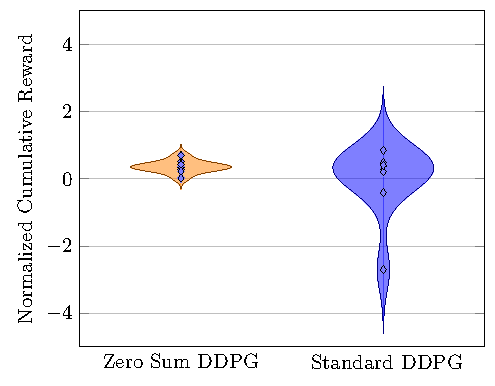
\includegraphics[width=0.6\textwidth]{plots/ddpg/violin_plot/initial_condition_shift}
	\caption{مقایسه مجموع پاداش دو الگوریتم تک‌عاملی و چندعاملی \lr{DDPG} در شرایط اولیه تصادفی}
\end{figure}

\begin{figure}[H]
	\centering
	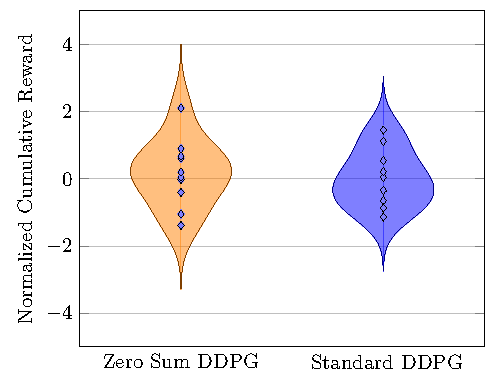
\includegraphics[width=0.6\textwidth]{plots/ddpg/violin_plot/actuator_disturbance}
	\caption{مقایسه مجموع پاداش دو الگوریتم تک‌عاملی و چندعاملی \lr{DDPG} در حضور اغتشاش در عملگرها}
\end{figure}

\begin{figure}[H]
	\centering
	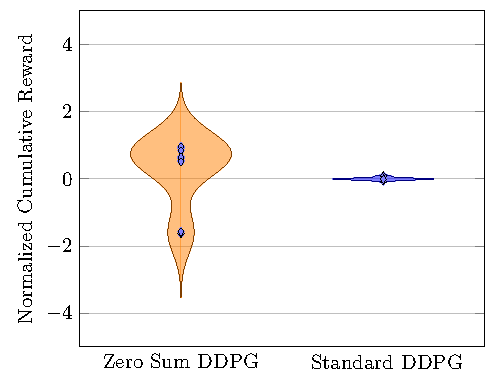
\includegraphics[width=0.6\textwidth]{plots/ddpg/violin_plot/model_mismatch}
	\caption{مقایسه مجموع پاداش دو الگوریتم تک‌عاملی و چندعاملی \lr{DDPG} در مواجهه با عدم تطابق مدل}
\end{figure}

\begin{figure}[H]
	\centering
	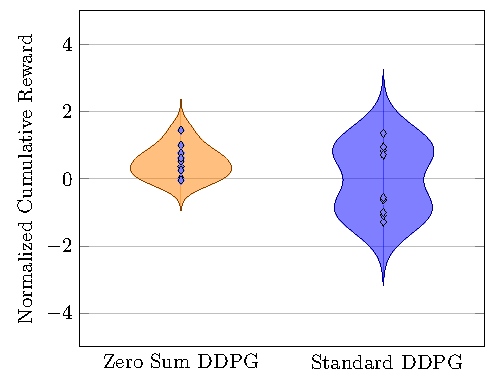
\includegraphics[width=0.6\textwidth]{plots/ddpg/violin_plot/partial_observation}
	\caption{مقایسه مجموع پاداش دو الگوریتم تک‌عاملی و چندعاملی \lr{DDPG} در شرایط مشاهده ناقص}
\end{figure}

\begin{figure}[H]
	\centering
	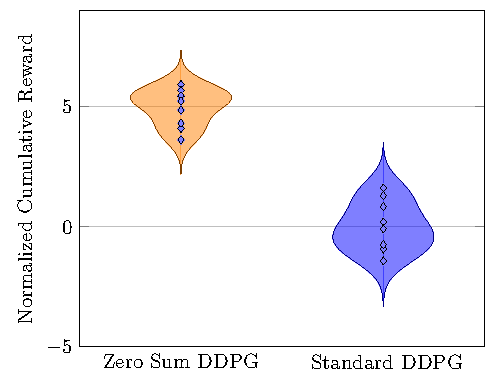
\includegraphics[width=0.6\textwidth]{plots/ddpg/violin_plot/sensor_noise}
	\caption{مقایسه مجموع پاداش دو الگوریتم تک‌عاملی و چندعاملی \lr{DDPG} در حضور نویز حسگر}
\end{figure}

\begin{figure}[H]
	\centering
	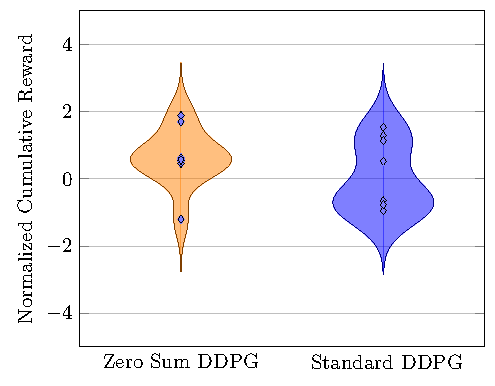
\includegraphics[width=0.6\textwidth]{plots/ddpg/violin_plot/time_delay}
	\caption{مقایسه مجموع پاداش دو الگوریتم تک‌عاملی و چندعاملی \lr{DDPG} در شرایط تأخیر زمانی}
\end{figure}



\begin{figure}[H]
	\centering
	
	% سطر اول
	\subfloat[شرایط اولیه تصادفی]{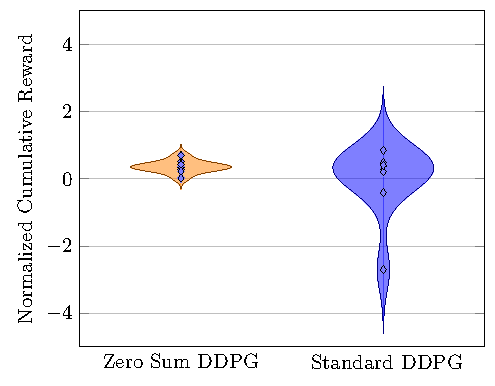
\includegraphics[width=.33\textwidth]{plots/ddpg/violin_plot/initial_condition_shift.pdf}}%
	\subfloat[اغتشاش در عملگرها]{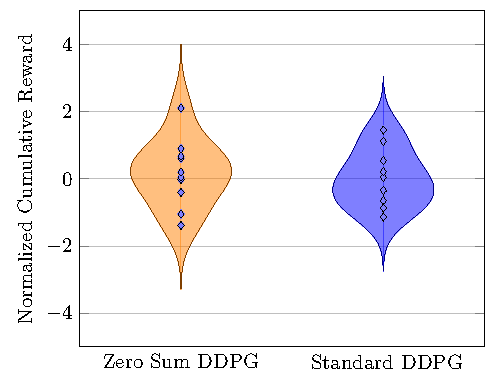
\includegraphics[width=.33\textwidth]{plots/ddpg/violin_plot/actuator_disturbance.pdf}}%
	\subfloat[عدم تطابق مدل]{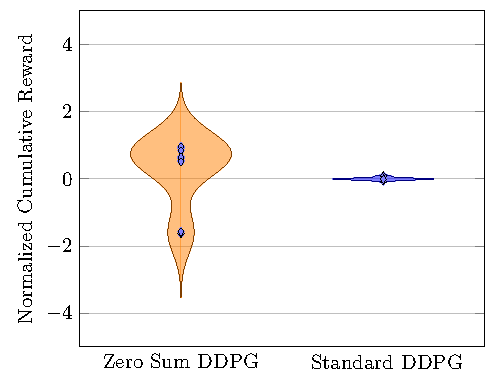
\includegraphics[width=.33\textwidth]{plots/ddpg/violin_plot/model_mismatch.pdf}}\\[1ex]
	
	% سطر دوم
	\subfloat[مشاهده ناقص]{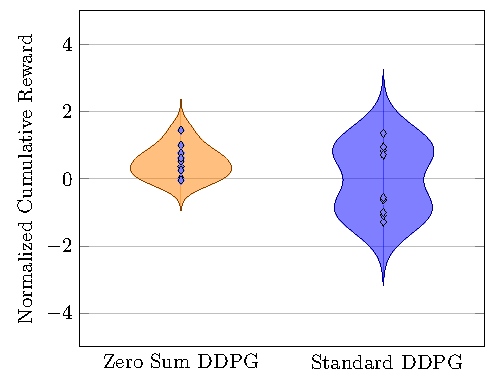
\includegraphics[width=.33\textwidth]{plots/ddpg/violin_plot/partial_observation.pdf}}%
	\subfloat[نویز حسگر]{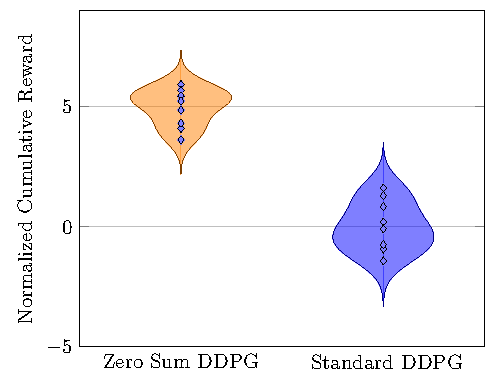
\includegraphics[width=.33\textwidth]{plots/ddpg/violin_plot/sensor_noise.pdf}}%
	\subfloat[تأخیر زمانی]{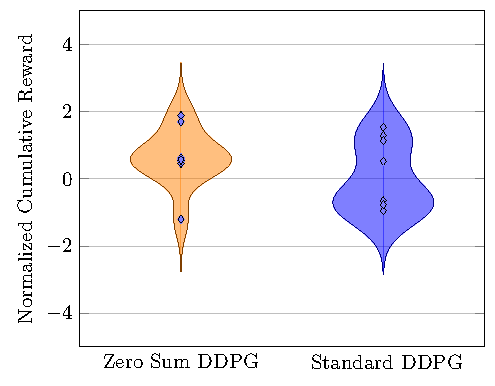
\includegraphics[width=.33\textwidth]{plots/ddpg/violin_plot/time_delay.pdf}}
	
	\caption{مقایسه مجموع پاداش دو الگوریتم تک‌عاملی و چندعاملی \lr{DDPG} در سناریوهای مختلف}
	\label{fig:ddpg_robustness_violin}
\end{figure}




\begin{figure}[H]
	\centering
	
	% سطر اول
	\subfloat[شرایط اولیه تصادفی]{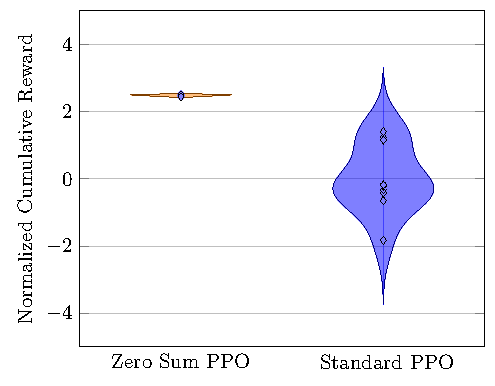
\includegraphics[width=.33\textwidth]{plots/ppo/violin_plot/initial_condition_shift.pdf}}%
	\subfloat[اغتشاش در عملگرها]{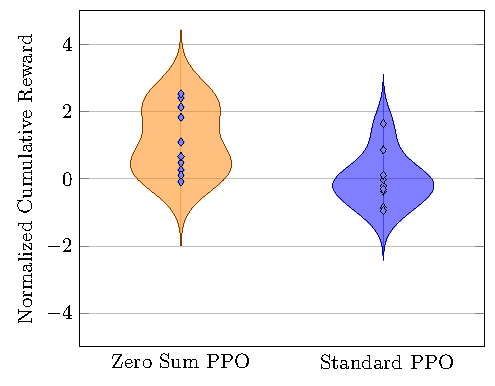
\includegraphics[width=.33\textwidth]{plots/ppo/violin_plot/actuator_disturbance.pdf}}%
	\subfloat[عدم تطابق مدل]{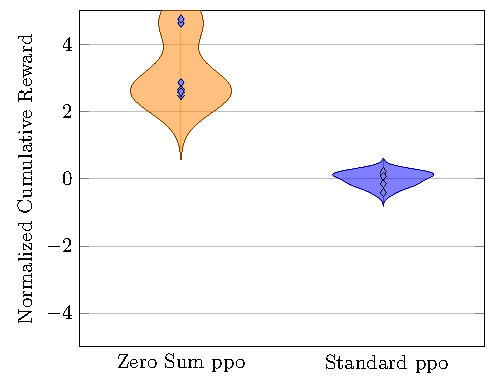
\includegraphics[width=.33\textwidth]{plots/ppo/violin_plot/model_mismatch.pdf}}\\[1ex]
	
	% سطر دوم
	\subfloat[مشاهده ناقص]{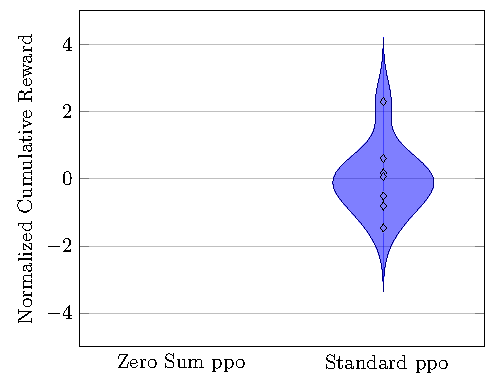
\includegraphics[width=.33\textwidth]{plots/ppo/violin_plot/partial_observation.pdf}}%
	\subfloat[نویز حسگر]{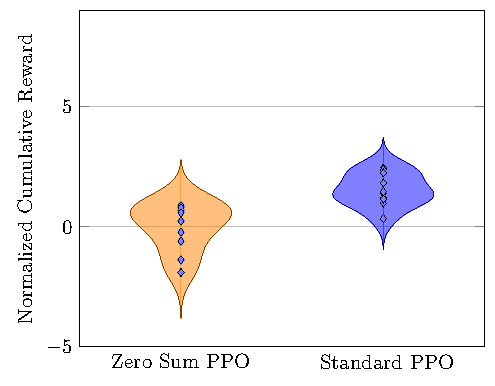
\includegraphics[width=.33\textwidth]{plots/ppo/violin_plot/sensor_noise.pdf}}%
	\subfloat[تأخیر زمانی]{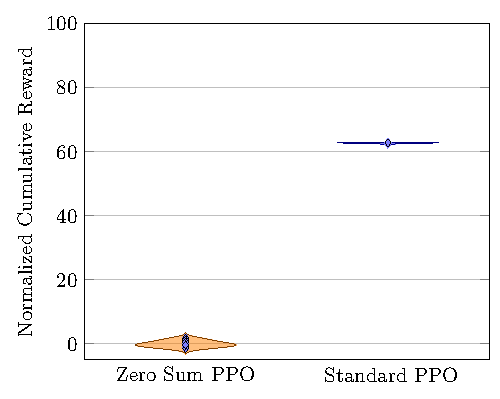
\includegraphics[width=.33\textwidth]{plots/ppo/violin_plot/time_delay.pdf}}
	
	\caption{مقایسه مجموع پاداش دو الگوریتم تک‌عاملی و چندعاملی \lr{PPO} در سناریوهای مختلف}
	\label{fig:ppo_robustness_violin}
\end{figure}





\begin{figure}[H]
	\centering
	
	% سطر اول
	\subfloat[شرایط اولیه تصادفی]{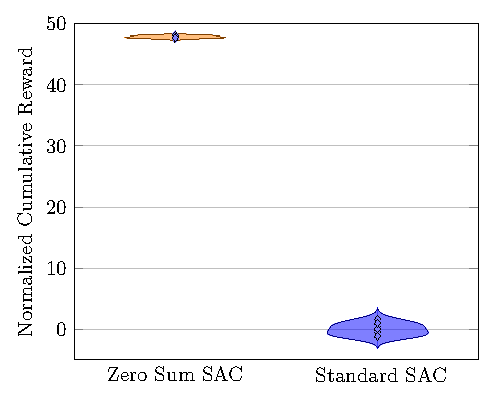
\includegraphics[width=.33\textwidth]{plots/sac/violin_plot/initial_condition_shift.pdf}}%
	\subfloat[اغتشاش در عملگرها]{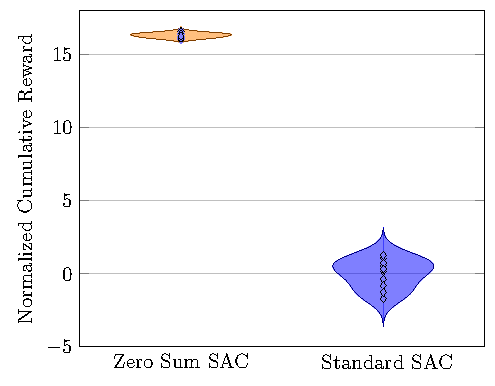
\includegraphics[width=.33\textwidth]{plots/sac/violin_plot/actuator_disturbance.pdf}}%
	\subfloat[عدم تطابق مدل]{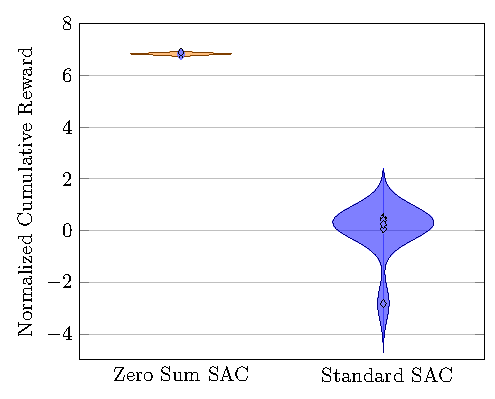
\includegraphics[width=.33\textwidth]{plots/sac/violin_plot/model_mismatch.pdf}}\\[1ex]
	
	% سطر دوم
	\subfloat[مشاهده ناقص]{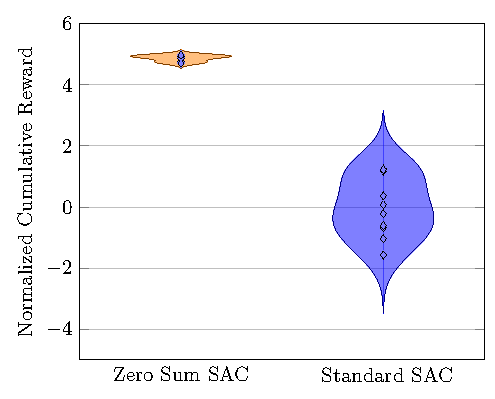
\includegraphics[width=.33\textwidth]{plots/sac/violin_plot/partial_observation.pdf}}%
	\subfloat[نویز حسگر]{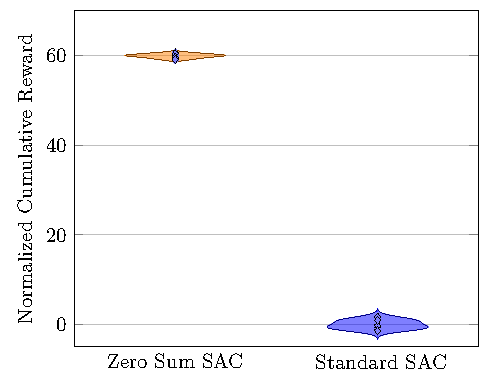
\includegraphics[width=.33\textwidth]{plots/sac/violin_plot/sensor_noise.pdf}}%
	\subfloat[تأخیر زمانی]{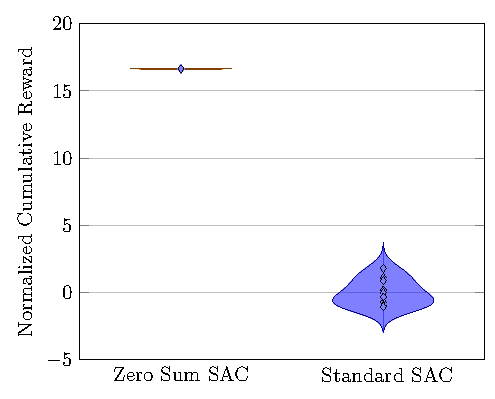
\includegraphics[width=.33\textwidth]{plots/sac/violin_plot/time_delay.pdf}}
	
	\caption{مقایسه مجموع پاداش دو الگوریتم تک‌عاملی و چندعاملی \lr{SAC} در سناریوهای مختلف}
	\label{fig:sac_robustness_violin}
\end{figure}